\chapter{Bridge}
\section{Intento}

Disaccoppia un'astrazione dalla sua implementazione in modo che i due possano variare indipendentemente. Per esempio nel caso di utilizzo di librerie esterne.

(nel progetto lo usiamo per isolare le librerie per inviare email e creare pdf)


%---
\section{Prestruttura}

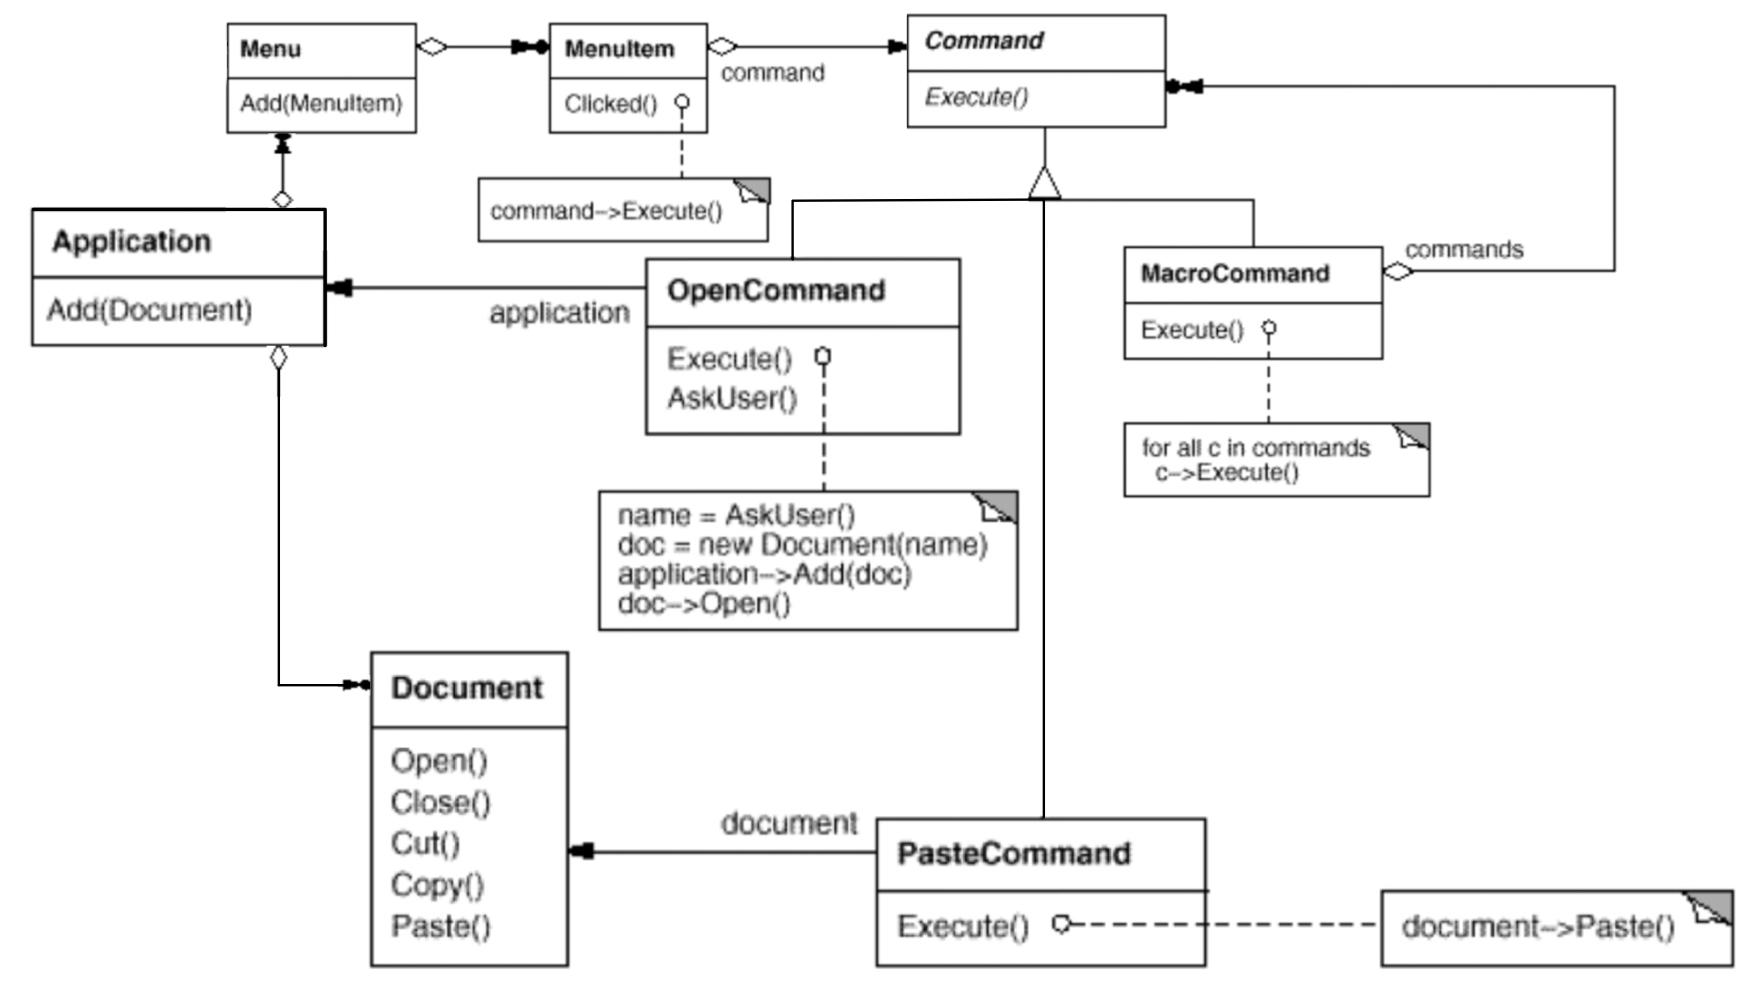
\includegraphics[width=\textwidth]{/Users/matt/Documents/GitHub/Design-Pattern-ITA/Bridge/Prestructure1}


%---
\section{Struttura}

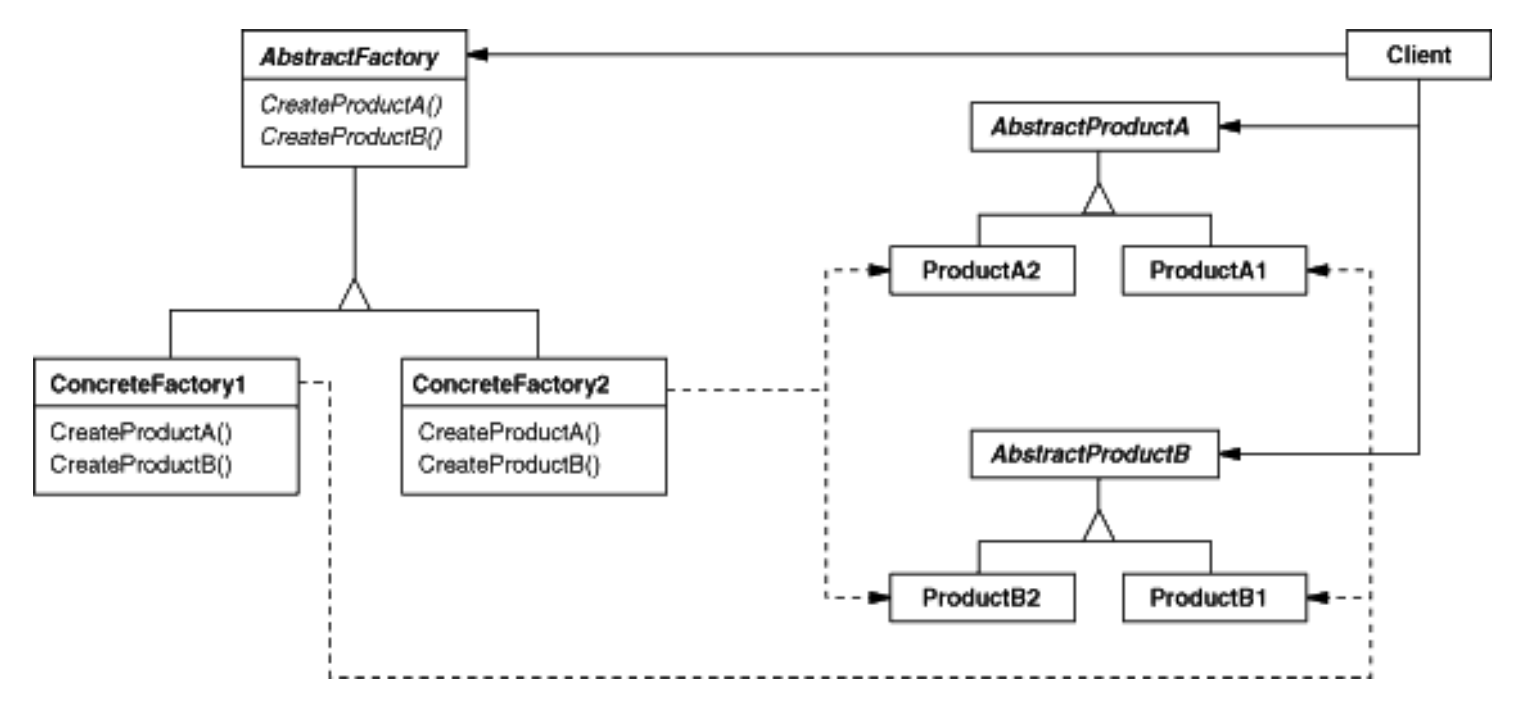
\includegraphics[width=\textwidth]{/Users/matt/Documents/GitHub/Design-Pattern-ITA/Bridge/Structure1}


%---
\section{Implementazione}

\subsection{Solo un implementazione.}
Se abbiamo solo un'implementazione, non è necessario creare una classe Implementor astratta. In tal caso ci sarà una relazione uno a uno tra Abstraction e Implementor.

Questa separazione è ancora utile quando una modifica nell'implementazione di una classe non deve influenzare i suoi client esistenti.

\subsection{Creazione dell'oggetto Implementor corretto.}
Come, quando e dove decidi quale classe Implementor istanziare quando ce n'è più di una?

Un'implementazione di elenchi collegati può essere utilizzata per piccole raccolte e una tabella hash per quelle più grandi.

Un altro approccio consiste nello scegliere inizialmente un'implementazione predefinita e modificarla in seguito in base all'utilizzo.

Oppure si può delegare del tutto la decisione ad un altro oggetto. Nell'esempio Window / WindowImp, possiamo introdurre un oggetto Factory il cui unico compito è incapsulare le specifiche della piattaforma.

La factory sa che tipo di oggetto WindowImp creare per la piattaforma in uso; a Window gli chiede semplicemente un WindowImp e restituisce il tipo giusto.


%---
\section{Esempio Java}
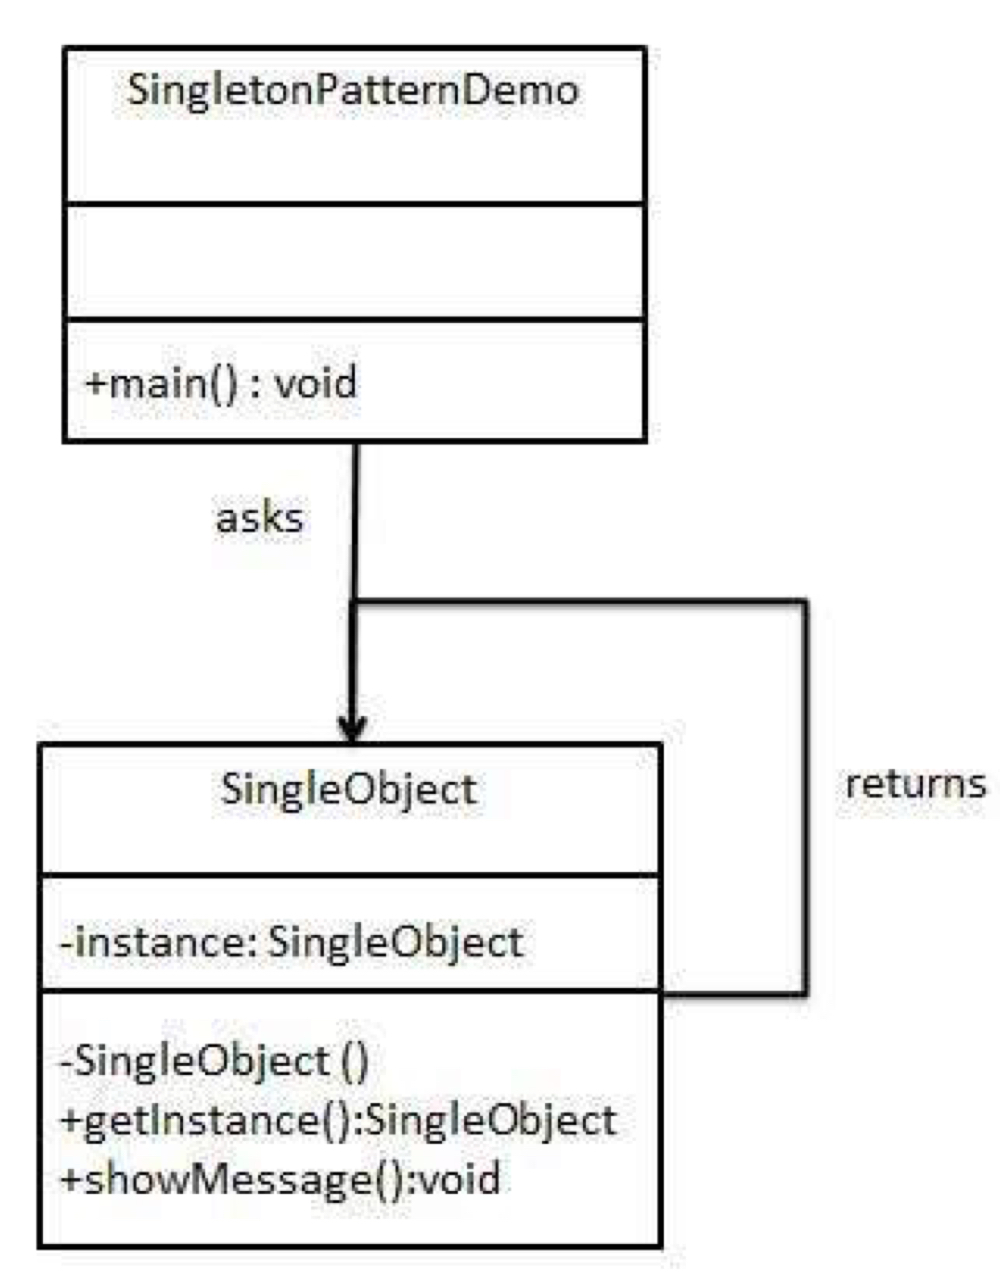
\includegraphics[width=\textwidth]{/Users/matt/Documents/GitHub/Design-Pattern-ITA/Bridge/Example1}

\subsection{DrawImplementation.java}
\begin{lstlisting}[language=java]
    public interface DrawImplementation {
        public void drawCircle(int x, int y, int radius);
    }
\end{lstlisting}

\subsection{Shape.java}
\begin{lstlisting}[language=java]
    public abstract class Shape {
        protected DrawImplementation drawImpl;
    
        protected Shape(DrawImplementation drawAPI) {
            this.drawImpl = drawAPI;
        }
    
        public abstract void draw();
    }
\end{lstlisting}

\subsection{Circle.java}
\begin{lstlisting}[language=java]
    public class Circle extends Shape{
        private int x, y, radius;
    
        public Circle(DrawImplementation drawImpl, int x, int y, int radius) {
            super(drawImpl);
            this.x = x;
            this.y = y;
            this.radius = radius;
        }
    
        @Override
        public void draw() {
            // specifico dell'ambiente windowing usato a runtime
            drawImpl.drawCircle(x, y, radius);
        }
    }
\end{lstlisting}

\subsection{RedCircle.java}
\begin{lstlisting}[language=java]
    public class RedCircle implements DrawImplementation{

        @Override
        public void drawCircle(int x, int y, int radius) {
            System.out.println("cerchio rosso di: " + radius + x + y);    
        }
        
    }
\end{lstlisting}

\subsection{GreenCircle.java}
\begin{lstlisting}[language=java]
    public class GreenCircle implements DrawImplementation{

        @Override
        public void drawCircle(int x, int y, int radius) {
            System.out.println("cerchio verde di: " + radius + x + y);    
        }
        
    }
\end{lstlisting}

\subsection{main}
\begin{lstlisting}[language=java]
    public static void main(String[] args) {
        Shape redC = new Circle(new RedCircle(), 100, 100, 10);
        Shape greC = new Circle(new GreenCircle(), 100, 100, 10);
    
        redC.draw();
        greC.draw();
    }
\end{lstlisting}